% Otto-von-Guericke-Universität Magdeburg
% Fakultät für Mathematik
%
% Vorschlag zur Gestaltung von Abschlussarbeiten mit LaTeX
%
%
%\documentclass[a4paper, 12pt]{scrreprt} % KOMA-Script-Report
%
\documentclass[a4paper, 12pt]{scrartcl} % KOMA-Script-Article 
%                                      (dann keine \chapter möglich!!!)
%                                      (erfodert Anpassung in FMA-commands.tex) 
%----LaTeX-Pakete-----------------
\usepackage[ngerman,american]{babel}   %Ueberschriften in Englisch
%\usepackage[american,ngerman]{babel}  %Ueberschriften in Deutsch
\usepackage[utf8x]{inputenc} % Quelltext mit Umlauteingabe

\usepackage{geometry}
\geometry{twoside, outer=25mm, inner=30mm, top=30mm, bottom=30mm} % zweiseitig
% \geometry{outer=25mm, inner=30mm, top=30mm, bottom=30mm}        % einseitig
\usepackage{latexsym}          % spezielle Mathematik-Symbole
\usepackage{graphicx}          % zum Einbinden von Bildern
\usepackage{amsmath, amssymb}  % LaTeX-Erweiterungen der AMS

% ----Einbinden von pdf-Dateien oder einzelnen Seiten daraus
\usepackage{pdfpages}
\usepackage{xspace}
\usepackage{setspace}        % zum Variieren des Zeilenabstandes
% Anwendung im Text:  \includepdf[pages={7, 9-12}]{Name der pdf-Datei}
%------
% Kopf- und Fußzeilen mit scrpage2 ---------------*Beginn*------------
\usepackage[automark,headsepline]{scrpage2}
\automark[section]{chapter}
\pagestyle{scrheadings}			
\clearscrheadfoot
\ihead[]{\headmark}
\cfoot[\hfill -- \thepage{} -- \hfill]{\hfill -- \thepage{} -- \hfill}
\setkomafont{pagefoot}{\normalfont\sffamily}
% Kopf- und Fußzeilen mit scrpage2 ---------------*Ende* --------------
\setlength{\parindent}{0cm}
\setcounter{tocdepth}{4}       % 4 Gliederungsebenen in das Inhaltsverzeichnis
\setcounter{secnumdepth}{3}    % 4 (!) Gliederungsebenen werden nummeriert(0-3) 
% zusätzliche LaTeX-Umgebungen und -Kommandos
% bei Bedarf aendern/ergänzen
%
% Definition von Umgebungen -----------------------------
%\newtheorem{theorem}{Theorem}[chapter]
\newtheorem{theorem}{Theorem}[section]   % falls scrartcl
\newtheorem{lemma}[theorem]{Lemma}
%\newtheorem{defi}{Definition}[chapter]
\newtheorem{defi}{Definition}[section]   % falls scrartcl 
%\newtheorem{example}{Beispiel}[chapter]
\newtheorem{example}{Beispiel}[section]  % falls scrartcl
%---------abkuerzenden Kommandos----------------------
\newcommand{\qed}{\qquad \hfill \fbox{}\\}
\newcommand{\qede}{\qquad \hfill \fbox{}}
\newcommand{\ew}{\mbox{\textbf{E}}}
\newcommand{\var}{\mbox{\textbf{Var}}}
\newcommand{\cov}{\mbox{\textbf{Cov}}}
\newcommand{\cor}{\mbox{\textbf{Corr}}}
\newcommand{\wra}{$(\Omega,\mathfrak{A},P)$ }
\newcommand{\A}{\mathfrak{A}}
\newcommand{\F}{\mathfrak{F}}
\newcommand{\D}[1]{\, \mathrm{d} #1}   % Integral d gerade Bsp.: dx --> \D{x}
\newcommand{\zB}{\mbox{z.\,B.}\xspace}
\newcommand{\dH}{\mbox{d.\,h.}\xspace}           % hilfreiche LaTeX-Befehlsabkürzungen
% ------------------------------------------------------------------------------
%
%###############################################################################
\begin{document}
\pagenumbering{Roman}
% Deckblatt der Abschlussarbeit
% nichts von der Formatierung verändern
%
% Einträge nur unterhalb der Zeile 
%####### hier aktualisieren
% bearbeiten
%
%

\begin{titlepage}
  \begin{center}
    \vspace*{1,5cm}
    \begin{Large}
      \doublespacing
      \begin{scshape}
        % ####### hier aktualisieren
        Julia : A Fresh Approach to Numerical Computation
      \end{scshape}
      \singlespacing
    \end{Large}
    \vspace{\fill}
    Faculty of Mathematics\\
    Otto-von-Guericke-Universität Magdeburg\\
    %zur Erlangung des akademischen Grades \\
    % Diplom-Mathematiker Diplom-Wirtschaftsmathematiker
    % Diplom-Technomathematiker Diplom-Computermathematiker
    %Bachelor of Science
    % Master of Science
    %\\
    %angefertigte\\
    \vspace{\fill}
    \begin{Large}
      % ####### hier aktualisieren durch Umsetzen des Kommentarzeichens %
      \textsc{Scientific Computation Seminar 2021}
      % \textsc{Bachelorarbeit}
      % \textbf{Diplomarbeit} \textbf{Masterarbeit}
      \\
    \end{Large}
    \vspace{\fill}

    by\\
    \textsc{Carl Julius Martensen}\\
    born on 31.10.1986, Preetz,\\
    %Studiengang Mathematik,\\
    %Studienrichtung Wirtschaftsmathematik.\\[2ex]
    \today\\
    \vspace{\fill} Supervised at the Max-Planck-Institut für Dynamik komplexer
    technischer Systeme
    % Algebra und Geometrie
    % Analysis und Numerik
    % Mathematische Optimierung Mathematische Stochastik
    by\\
    \begin{scshape}
      Dr. Jens Saak
    \end{scshape}
  \end{center}
\end{titlepage}

%%% Local Variables: 
%%% mode: latex
%%% TeX-master: "FMA-Vorlage"
%%% TeX-PDF-mode:t
%%% auto-fill-function:nil
%%% mode:auto-fill
%%% flyspell-mode:nil
%%% mode:flyspell
%%% ispell-local-dictionary: "american"
%%% End: 


\tableofcontents
\clearpage
% \addcontentsline{toc}{section}{Abbildungsverzeichnis}
% \listoffigures
% \cleardoublepage
\pagenumbering{arabic}
\setcounter{page}{1}      %Beginn der Textseitenzaehlung
% ------------------------------------------------------------------------------
% hier beginnen die einzelnen Kapitel der Arbeit
% The following text is only demonstrating the use of sections for structuring
% the contents. The section names are by no means obligatory.

\section{Introduction}
\label{JM:sec:introduction}

In the world of today's sciences, the use of computers has transformed the field and requirements for researchers tremendously. 
The ability to collect and process data at high rates using (semi-) automatic approaches pushes the classical research fields like
physics, biology, medicine, engineering, and social sciences towards hybrid models and big data evaluation. A recent example is the detection of gravitational waves, 
where multiple software components have been used to process the data and help the researchers to classify the events \cite{JMMacleodEtAl2021} .\\


The requirements on software development used for research purposes have decreased below expert knowledge. Research software and coding are much more of a general tool, similar to text editors, for many scientific disciplines. 
As a result scientists from fields where programming and numerical computation play at most a minor role, e.g. psychology, sociology but also biology, start to develop code on their own.
This is reflected in the rise of high-level languages like \textit{Python}, \textit{Ruby}, \textit{R}, or \textit{Lua} \cite{JMVanRossumDrake2009,JMThomasEtAl2005, JMRCT2016, JMIerusalimschy2006} which are semantically easier to program as opposed to lower-level languages such as 
\textit{C}, \textit{C++}, \textit{Fortran}, \textit{Go}, and \textit{Rust} \cite{JMKernighanRitchie2006, JMStroustrup2013, JMBackusHeising1964, JMMeyerson2014, JMMatsakisKlockII2014}. 
The broader, more diverse user base of high level languages results in a more versatile ecosystem, giving rise to various packages and modules designed
for specific tasks with a clean interface. Despise these advantages, the price to be paid is commonly linked to the performance in terms of execution time and memory consumption of the resulting code. 
A common pattern used is hence to write an application programming interface (API) in high-level languages and move the computationally expensive parts to a low-level implementation after finishing prototyping. 
This is referred to as the \textit{two language problem}.
This approach, while being general, has some major drawbacks related to datatype availability, effort of maintanance, and dependency management - to name just a few.\\

To resolve this - and other - problems of scientific computation the \textit{Julia} programming language has been created \cite{JMBezansonEtAl2015}. It aims to provide performant code, leveraging the best features of 
prominent languages without complicated semantic structures, contradicting the common misconception that computational performance comes at the price of ease of use \cite{JMEdelman2019}. 
Even though being a relatively new language, initially released in 2012 for the broader public, \textit{Julia} gained much momentum over the last five decade, being used in various scientific disciplines CITE. \\

In the following, \textit{Julia} will be introduced as a language for scientifc computation. Section \ref{JM:sec:basics} starts by introducing how to define and analyse functions before introducing the concept of multiple dispatch to the reader.
Afterward, section \ref{JM:sec:JITOpt} explains benchmarking, optimizing code, and just-in-time compilation. Section \ref{JM:sec:GOMP} a simple greedy algorithm for sparse regression is implemented, showcasing the ease of use to transpile mathematical notation to fast code.
Section \ref{JM:sec:ECO} highlights some of the most useful and prominent packages of the language.
A conclusion is drawn in section \ref{JM:sec:CONC}.

\newpage

\section{Basics and Multiple Dispatch}
\label{JM:sec:basics}

There exist different ways to define functions in \text{Julia}. Similar to e.g. \text{Python} or \text{Matlab}, a simple Gaussian radial basis function $f : \mathbb{R} \times \mathbb{R} \mapsto \mathbb{R}$ 
can be implemented as follows

\lstinputlisting[language=Julia,firstline=1, lastline=8]{../scripts/HelloWorld.jl}

As we can see, we defined no input types for the function and called it with a Float64 and Int64 as arguments, resulting in a Float64 as the best intersection of both number types.
Changing the input type of the first argument to Float32 returns Float32, again using the intersection of the input data types. To see how the evaluation works, we will use

\lstinputlisting[language=Julia,firstline=10, lastline=10]{../scripts/HelloWorld.jl}

Which will evaluate the function and returns a lowered and type-inferred abstract syntax tree for the method

\begin{lstlisting}[language=Julia]
    CodeInfo(
        1 ─ %1 = Base.sitofp(Float64, y)::Float64
        │   %2 = Base.sub_float(x, %1)::Float64
        │   %3 = Base.mul_float(%2, %2)::Float64
        │   %4 = Base.neg_float(%3)::Float64
        │   %5 = invoke Main.exp(%4::Float64)::Float64
        └──      return %5
        ) => Float64
\end{lstlisting}

The above output contains two important informations: the intermediate representation (IR), indicated by the lines with a leading \%, passed on to the compiler and the type information
propagated through the function. 
It first the value of $y$ is converted into a Float64 (\%1), the difference $x-y$ is computed (\%2), multiplied with itsself (\%3), negated (\%4) and mapped via the exponential function (\%5).
Entering different arguments also works out of the box. Using a pair of ComplexFloat64 and Float32 
returns a complex-valued result, as can be expected. 
Different representations as the one shown above can be accessed via {@code\_lowered}, @{code\_typed}, @{code\_lowered} and @{code\_native}. These return the IR, IR with type information, the code for the compiler and the machine code respectively.

\lstinputlisting[language=Julia,firstline=12, lastline=12]{../scripts/HelloWorld.jl}

The reason why this approach works is called multiple dispatch (MD) and a core design element of \textit{Julia}. Most prominent languages operate on
obect-oriented programming (OOP) or use functional programming\footnote{FP refers to purely functional programming in the scope of this work. In general modern languages using FP as a paradigm, like \textit{Closure}, tend to use MD.} (FP).
In FP, each function is defined uniquely by its name and stored in the global namespace. OOP stores methods related to objects in the namespace
of the corresponding object definition, allowing for more expressiveness and clarity in defining the functions.

Following \cite{JMKarpinski2019}, the expressiveness of a language can be defined as the number of different methods with the same name but different purposes depending on their arguments.
Consider the exponential function $exp : \mathbb{X} \mapsto \mathbb{X},~ \mathbb{X} \in \lbrace \mathbb{R}, \mathbb{C}, \dots \rbrace$. FP would define several methods by name for different 
arguments, e.g. $exp_{\mathbb{R}}$, $exp_{\mathbb{C}}$. In OOP, the object itself is the dispatch argument, so a pseudo-code notation would result in $\mathbb{R}.exp$, $\mathbb{C}.exp$.
In MD, all input arguments are checked, hence $exp$ can be used and extended for all types it holds a definition for. These insights are summarized in Table \ref{JM:tab:ExpressivePow}, showing the proportional
growth of expressiveness in relation to their dispatch arguments. \\

\begin{table}
    \begin{tabular}{|l|l|l|l|} \hline
        & FP & OOP & MD \\ \hline
        Dispatch arguments & $\emptyset$ & $\lbrace x_1 \rbrace$ & $\lbrace x_1 , x_2, \dots, x_N \rbrace$ \\
        Expressive Order &  $\mathcal{O}\left(1\right)$ & $\mathcal{O}\left(\left|x_1\right|\right)$ &  $\mathcal{O}\left(\prod_{i=1}^N \left|x_i\right|\right)$ \\
        Expressive Power & const. & linear & exponential \\ \hline
    \end{tabular}
    \caption{Expressiveness of different programming paradigms}
    \label{JM:tab:ExpressivePow}
\end{table}

If a general function, e.g. $+$, is called in \textit{Julia}, the compiler automatically uses the right function definition based on the arguments. 
This can be confirmed with


\begin{lstlisting}[language=Julia]
    methods(+, (Number,Number))
    # 40 methods for generic function "+":
    [1] +(x::T, y::T) where T<:Union{Int128, ..., UInt8} in Base at int.jl:87
    [2] +(c::Union{UInt16, UInt32, UInt64, UInt8}, x::BigInt) in Base.GMP at gmp.jl:528
    [3] +(c::Union{Int16, Int32, Int64, Int8}, x::BigInt) in Base.GMP at gmp.jl:534
    [4] +(c::Union{UInt16, UInt32, UInt64, UInt8}, x::BigFloat) in Base.MPFR at mpfr.jl:376
    [5] +(c::Union{Int16, Int32, Int64, Int8}, x::BigFloat) in Base.MPFR at mpfr.jl:384
    [6] +(c::Union{Float16, Float32, Float64}, x::BigFloat) in Base.MPFR at mpfr.jl:392
    ... 
\end{lstlisting}

which returns all methods defined in the current workspace for the $+$ operator using two Number types as inputs. Number represents an abstract type spanning various number types, e.g. Float, Int, UInt, Complex. 
Evaluating the following code block 

\lstinputlisting[language=Julia,firstline=14, lastline=16]{../scripts/HelloWorld.jl}

returns the corresponding method used for computation and where it is defined.

\begin{lstlisting}[language=Julia]
    exp(x::T) where T<:Float32 in Base.Math at special/exp.jl:229
    exp(z::Complex) in Base at complex.jl:638
\end{lstlisting}

A key difference to OOP based programming is that no method definition has to explicitly know of the other, as long as it is unique in its dispatch arguments\footnote{An unwanted dispatch on an already defined method can result unstable behaviour and called \textit{type-piracy}}.
This allows developers to easily extend existing packages and functionalities, allowing excessive reuse of the codebase\footnote{A good example is given by \url{https://github.com/JuliaPlots/RecipesBase.jl}, which is used to define individual recipes used for plotting without explicitly depending on \textit{Plots.jl}}. 
As a small example consider defining a new Number type and its corresponding $\exp$:

\lstinputlisting[language=Julia,firstline=19, lastline=27]{../scripts/HelloWorld.jl}

To make the function $f$ useable for vector operations, multiple dispatch can be leveraged as well:

\lstinputlisting[language=Julia,firstline=29, lastline=38]{../scripts/HelloWorld.jl}

Since both $\exp$ and \^~ are not defined for vectors, we use broadcasting to call the function on each element of the data structure individually. This is accomplished via the 
. operator. Checking the available definitions of the function via 

\lstinputlisting[language=Julia,firstline=40, lastline=40]{../scripts/HelloWorld.jl}

we can see that two definitions are present

\begin{lstlisting}[language=Julia]
    # 2 methods for generic function "f":
    [1] f(x::AbstractVector{T} where T, y::AbstractVector{T} where T) in Main at ./HelloWorld.jl:32
    [2] f(x, y) in Main at ./HelloWorld.jl:3
\end{lstlisting}

[1] is the definition we just added and [2] our original implementation from the beginning of this section, extending the function to be reused and avoiding different naming schemes.

\newpage





%\input{contents/01_motivation.tex}
%\section{Design}
\section{ Just-In-Time Compilation and Optimizing Code}
\label{JM:sec:JITOpt}

A common complain of users new to \textit{Julia} is that is does not hold up to its promise of speed, often feels even slower than e.g. using \textit{Python} for the same 
task. This chapter gives a brief explanation on why this is the case, how performance should and can be measured, and how to optimize code for performance. Consider the following code

\lstinputlisting[language=Julia,firstline=1, lastline=15]{../scripts/optimizing_code.jl}

Where the @time macro\footnote{A macro transforms the AST of the program. A exhausting introduction has been given at JuliaCon 2021 CITE. Interested readers might also refer to \cite{JMKwong2020}.}
returns basic performance metrics about the function call like overall execution time, memory allocations and compilation time.

\begin{lstlisting}[language=Julia]
    0.016432 seconds (6.08 k allocations: 342.705 KiB, 99.78% compilation time)
\end{lstlisting}

Another execution of the same command holds a different result.

\begin{lstlisting}[language=Julia]
    0.000008 seconds (1 allocation: 160 bytes)
\end{lstlisting}

The reason is \textit{Julia}'s underlying just-in-time (JIT) compilation. On the first call of the method $g$, 
the code is lowered to machine instructions and stored in memory for the specific types of arguments. This means that the first 
call of a method has an additional overhead due to the effort of the LLVM \cite{JMLattnerAdve2004} compiler\footnote{Which is also the reason for the infamous time to first plot benchmark in \textit{Julia}}.
The second call of a method leverages the already compiled function and can be executed and benchmarked faster. A slight change of arguments shows that this process is indeed type specific.

\lstinputlisting[language=Julia,firstline=19, lastline=22]{../scripts/optimizing_code.jl}

Again, the compilation time is present and takes up most of the execution time

\begin{lstlisting}[language=Julia]
    0.100689 seconds (269.78 k allocations: 15.753 MiB, 10.07% gc time, 99.92% compilation time)
\end{lstlisting}

JIT compilation also exist for different languages, such as \textit{Python}, \textit{lua} or \textit{Matlab}\cite{JMMATLAB2010}, as an optional extension. However, most of the performance comes
from compiler optimization at which \textit{Julia} exceeds performance-wise due to JIT being the standard. 
A slightly outdated benchmark comparing different algorithms and languages can be found \href{https://julialang.org/benchmarks/}{at the micro-benchmark page.}\\

\textit{Julia} is storing array-like data in a column major memory layout, which highly impacts the speed. The execution of the following
code shows that a column major iteration can result in a high speedup, using the same array. 

\lstinputlisting[language=Julia,firstline=24, lastline=46]{../scripts/optimizing_code.jl}

Instead of using @time the performance metrics are derived via @btime \footnote{\href{https://github.com/JuliaCI/BenchmarkTools.jl}{BenchmarkTools.jl}}, which (possibly) evaluates the method over multiple trials.\\

To investiage the use of parallel processing, consider the example given in \cite[p. 178 ff.]{JMSengupta2019}

\lstinputlisting[language=Julia,firstline=49, lastline=68]{../scripts/optimizing_code.jl}

Both methods defined above are mutating, indicated by the exclamation mark at the end of the function. They modify the values of their first argument, the array $x$, overwriting it inplace with no further allocations.
We see that the use of the second function, which leverages single-instruction-multiple-data (SIMD) and neglecting bounds checking holds a relative speedup of $4.18$. A similar syntax enables multithreading

\lstinputlisting[language=Julia,firstline=74, lastline=83]{../scripts/optimizing_code.jl}

Which shows the ease of use, but the communication time dominates the execution time and no speedup is achieved. Likwise, computations can be moved from the CPU to the GPU using different pacakges \cite[p.204 ff.]{JMSengupta2019}.

















\section{Orthogonal Matching Pursuit}
\label{JM:sec:GOMP}

In the following section, preconditioned generalized orthogonal matching pursuit (GOMP) \cite{JMTongEtAl2020} will be implemented.
Matching pursuit algorithms are a class of greedy algorithms designed to solve the sparse signal recovery problem

\begin{equation}
\begin{aligned}
    \min_x \quad & \left\lVert x \right\rVert_0 \\
    \textrm{s.t.} \quad & y = \Psi x
\end{aligned}
\end{equation}

where $x \in \mathbb{R}^n$ is an unknown sparse signal, $\Psi \in \mathbb{R}^{m \times n}$ is called the sampling matrix and $y \in \mathbb{R}^m$
a measured signal. GOMP aims to find the best $K$-sparse support in the span of $\Psi$, iteratively reducing the estimation error of the recovered signal by selecting $S$ most similiar components.\\

The main algorithm can be described as follows

\begin{algorithm}[H]
    \SetAlgoLined
    \KwResult{$x$}
    \KwData{$y$, $\Psi$, $K$, $S = 1$}
    Projection onto span\; 
    $P = \Psi^T \left(\Psi\Psi^T\right)$;
    $\tilde{y} = P y$;
    $\tilde{\Psi} = P \Psi$\;
    Initialize residual and support\;
    $r = y$;
    $\Lambda = \emptyset$\;
    \While{Not converged}{
        $S = \delta_S\left( \left| \tilde{\Psi}^T~r \right| \right)$\;
        $\Lambda = \Lambda \cup S$\;
        $x = \min \left\lVert \tilde{y} - \tilde{\Psi}u \right\rVert_2~, \quad supp(u) = \Lambda$\;
        $r = \tilde{y} - \tilde{\Psi} x$\;
    };
\end{algorithm}

Where $\delta_S\left( x \right) : \mathbb{R}^n \mapsto \lbrace 0, 1 \rbrace^n$ denotes (with abuse of notation) the mapping of the $S$ largest elements onto a corresponding
indicator vector. A similar notation to the pseudocode above can be achieved in \textit{Julia}. For brevity, only necessary elements of the source code will be shown, which can be found in detail in REF. The function is defined as follows

\lstinputlisting[language=Julia,firstline=4, lastline=6]{../scripts/gomp.jl}

First, we will focus on the preconditioning via the matrix $P \in \mathbb{R}^{m \times m}$ mapping onto the
column span of $\Psi$

\lstinputlisting[language=Julia,firstline=22, lastline=26]{../scripts/gomp.jl}

Next, the iterative computation of the support, corresponding coefficients and residuals is performed

\lstinputlisting[language=Julia,firstline=37, lastline=50]{../scripts/gomp.jl}

The results of the algorithm are shown in Fig. \ref{JM:fig:GOMP}, where a 100 dimensional sparse vector has been recovered with varying noise level.

\begin{figure}
    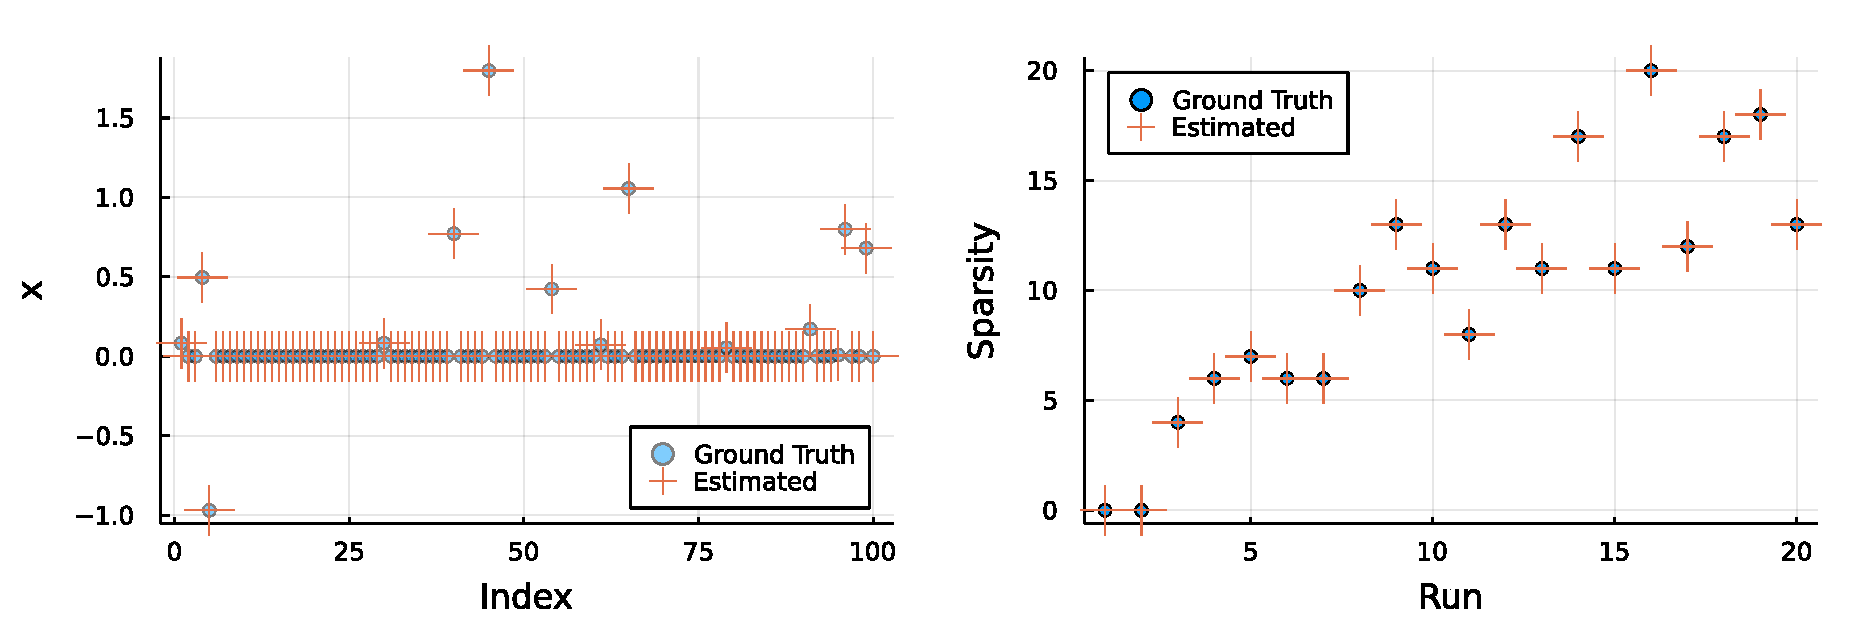
\includegraphics[width = 0.9\textwidth]{../figures/merged.pdf}
    \caption{Performance of GOMP for a sparse 100 dimensional vector (left) and with increasing noise level (right)}
    \label{JM:fig:GOMP}
\end{figure}

%\subsection{Basic Defintions and Notation}
%\label{sec:basic-defint-notat}

%\section{Basics}
%\label{sec:overview}

%\subsection{Multiple Dispatch versus Object Oriented Programming}

%\subsection{Just-In-Time And Precompilation}

%\subsection{Interoperability}

%\subsection{Ecosystem For Numerical And Scientific Computation}

%\section{Experiments}
%\label{sec:experiments}


%%% Local Variables: 
%%% mode: latex
%%% TeX-master: "FMA-Vorlage"
%%% TeX-PDF-mode:t
%%% auto-fill-function:nil
%%% mode:auto-fill
%%% flyspell-mode:nil
%%% mode:flyspell
%%% ispell-local-dictionary: "american"
%%% End: 

% 
\newpage

\section*{Erklärung}		
\thispagestyle{empty}				

Hiermit erkläre ich, dass ich die vorliegende Arbeit selbstständig und ohne
Benutzung anderer als der angegebenen Quellen und Hilfsmittel angefertigt habe.
\newline\newline 
Ort, Datum, Unterschrift
\end{document}
% for emacs user
%%% Local Variables: 
%%% mode:latex
%%% TeX-master:t
%%% TeX-PDF-mode:t
%%% auto-fill-function:nil
%%% mode:auto-fill
%%% flyspell-mode:nil
%%% mode:flyspell
%%% ispell-local-dictionary: "american"
%%% End: 
